% XCircuit output "crowbar.tex" for LaTeX input from crowbar.eps
\def\putbox#1#2#3#4{\makebox[0in][l]{\makebox[#1][l]{}\raisebox{\baselineskip}[0in][0in]{\raisebox{#2}[0in][0in]{\scalebox{#3}{#4}}}}}
\def\rightbox#1{\makebox[0in][r]{#1}}
\def\centbox#1{\makebox[0in]{#1}}
\def\topbox#1{\raisebox{-0.60\baselineskip}[0in][0in]{#1}}
\def\midbox#1{\raisebox{-0.20\baselineskip}[0in][0in]{#1}}
   \scalebox{1}{
   \normalsize
   \parbox{4.5625in}{
   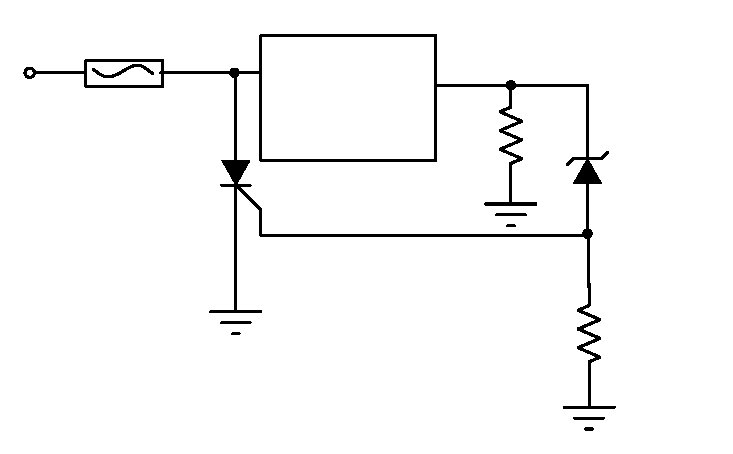
\includegraphics[scale=1]{crowbar}\\
   % translate x=558 y=152 scale 0.38
   \putbox{4.07in}{1.86in}{1.20}{Zener}%
   \putbox{4.07in}{1.61in}{1.20}{25V}%
   \putbox{4.07in}{1.36in}{1.20}{11V}%
   \putbox{0.44in}{2.62in}{1.20}{Fusible}%
   \putbox{2.94in}{1.93in}{1.20}{RL}%
   \putbox{1.87in}{2.23in}{1.20}{Circuito}%
   \putbox{0.70in}{1.88in}{1.20}{Tiristor}%
   \putbox{0.88in}{1.65in}{1.20}{9A}%
   \putbox{0.79in}{1.43in}{1.20}{(min)}%
   } % close 'parbox'
   } % close 'scalebox'
   \vspace{-\baselineskip} % this is not necessary, but looks better
